\section{History}
\label{intro:history}
The scattering of acoustic and electromagnetic waves by rough interfaces has been the subject of considerable study for more than a century \cite{varadan2013low}. Lord Rayleigh first investigated this problem in 1881 \cite{rayleigh1881x} and provided the foundation on which almost all subsequent work is based. It is possible to gain a good understanding of the mechanics of this field of scientific study and its application in light scattering by reading the works of van de Hülst (1957) \cite{hulst1981light}, Twersky (1964) \cite{twersky1964rayleigh}, Kerker (1969) \cite{Kerker1969TheSO}, Petit (1980) \cite{Petit80}, and Wilcox (1984) \cite{Wilcox84}. For the interested reader, we recommend the Habilitationsschrift of T. Arens (2009) \cite{ArensHab} as a definitive reference for periodic layered media problems and for the the state-of-the-art analysis of solutions to the Helmholtz and Maxwell equations in two and three dimensions.

Scattering is a process that alters the direction of light and is commonly associated with light's interaction with small particles \cite{choudhury2014principles}. Light scatters and travels in many directions other than the propagating direction as a result of this. Light is scattered by reflection and refraction in relatively large particles, such as pigments with dimensions greater than 2.0 $\mu$m. Diffraction occurs when light is scattered by relatively small particles with dimensions less than about 0.3 $\mu$m. When the sun is high in the sky during the day, the sky appears blue because blue light is scattered more effectively by very small particles in the atmosphere than light of longer wavelengths. When the sun is low on the horizon at sunrise and sunset, we see more of the non-scattered light, and the sky appears red. 

The majority of the objects we see are visible due to light scattering from their surfaces.  This is, after all, our fundamental physical observation method \cite{Kerker1969TheSO}. Light scattering is determined by the wavelength or frequency of the light being scattered. Because visible light has a wavelength on the order of a micron, objects much smaller than this cannot be seen, even with a microscope. Lord Rayleigh was among the first to explain light scattering by very
small particles. Rayleigh's observations show that the intensity of light scattered varies \cite{choudhury2014principles}:
\begin{itemize}
    \item Directly based on the intensity of incident light.
    \item Directly based on the average volume of scattering particles.
\end{itemize}
Lord Rayleigh also discovered that light can scatter without the use of scattering particles. This is due to the fact that changes in refractive index at different parts of a material can be sufficient to cause scattering. If a material is homogeneous, then the composition of all infinitesimal volume elements is the same and optical properties which define the material response to the incident radiation, such as transmissivity, reflectivity, and absorptivity are also the same. The aforementioned properties vary in different directions in a heterogeneous material, resulting in light scattering. On a macroscopic scale, optical properties vary over distances less than the wavelength of the incident light, resulting in the scattering of energy away from the direction of propagation. 

The result of Rayleigh's observations that scattering depends on the wavelength and, thus, the color of the light is  now known as the Rayleigh scattering law \cite{rayleigh1871scattering,lord1871light}. To answer the question: ``Why is the sky blue in the afternoon and red at sunset or sunrise?" one may observe that blue light has a wavelength of around 400 nanometers, while red light has a wavelength of about 700 nanometers. The scattering law states that the percentage of light that will be scattered is inversely proportional to the fourth power of the wavelength. Therefore, blue light, which is at the short wavelength end of the visible spectrum, will be scattered much more strongly than red light, which is at the long wavelength end of the visible spectrum. The white light from the sun scatters and splits into different components due to particles in our environment that are roughly the same size as the wavelength of visible light.
Because of their small size, oxygen and nitrogen (the major components of our atmosphere) scatter violet and blue light.  This results in the blue color of the afternoon sky, since, in directions other than towards the Sun, the observer sees predominantly scattered light. In contrast, the distance that light must travel from the Sun to an observer is highest at sunrise and dusk. This signifies that a substantial proportion of blue and violet light has been scattered, resulting in light that is predominantly of a longer wavelength and appears red to an observer. 
\vspace{-17mm}
\begin{figure}[H]
\centering
    \subfloat[Blue Sky (Afternoon)]
    {{
\includegraphics[width=7.15cm]{figures/blue_sky.png} }}
    \subfloat[Red Sky (Dawn and Dusk)]
    {{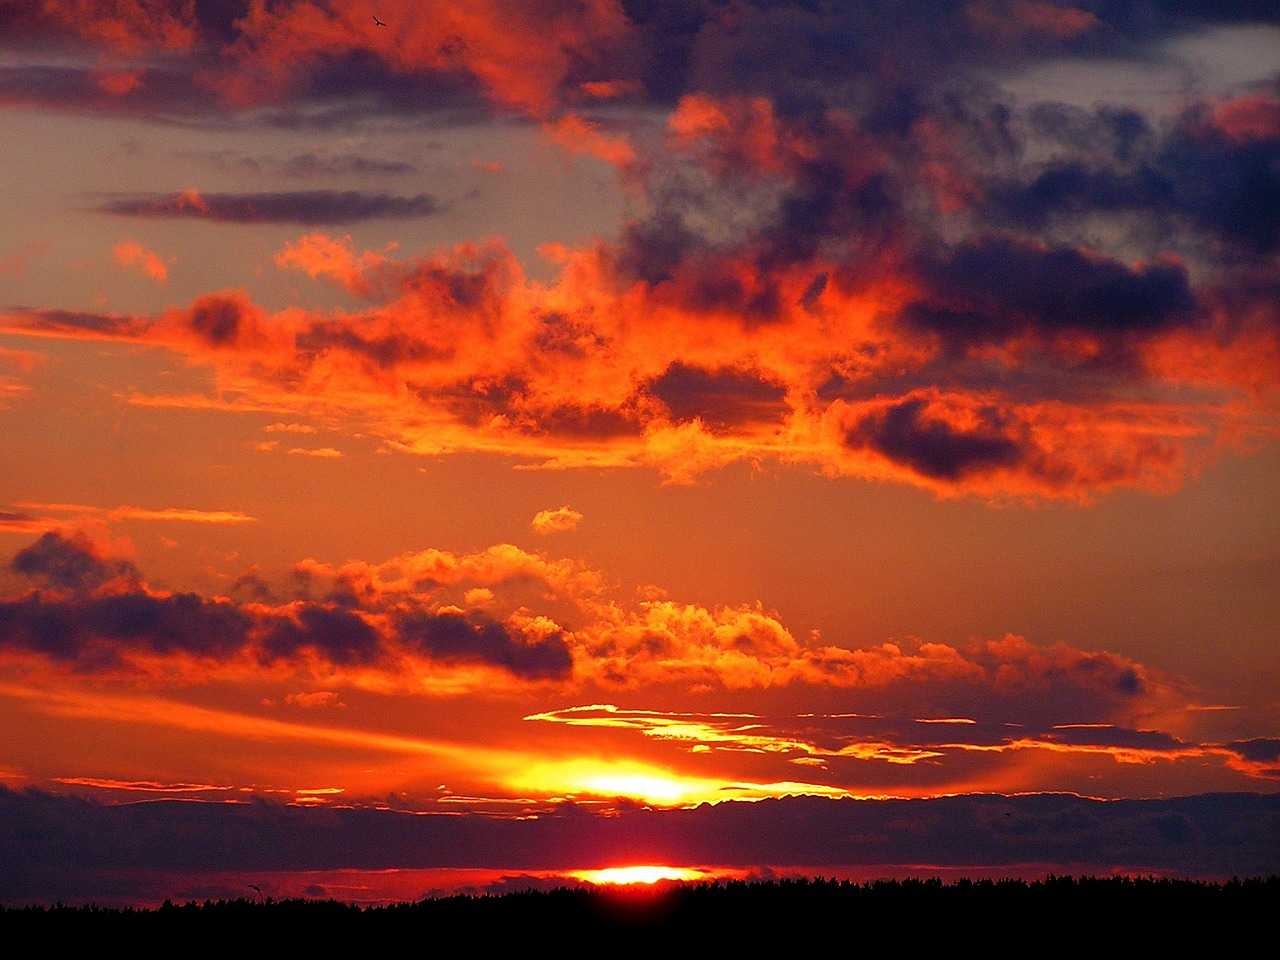
\includegraphics[width=7.15cm]{figures/red_sky.png} }}
%\includegraphics[width=0.5\textwidth]{conv_N}
\vspace{3mm}
\caption{Rayleigh scattering is responsible for the sky's blue tint during the day and the Sun's reddening at sunset and sunrise.}
%\label{Fig:N}
\end{figure}
\vspace{-18mm}
Research in the twentieth century focused on the subject of scattering from particles. In this, numerous authors contributed to the general theory of scattering by acoustic and electromagnetic waves. L. Foldy was among the first to present a complete framework \cite{foldy1945multiple} for the multiple scattering of a random distribution of particles. He considered the multiple scattering of scalar waves by a random distribution of isotropic scatterers through averaging a medium of uncorrelated, isotropic, point scatterers. M. Lax then expanded Foldy's work by including anisotropic scattering and pairwise correlation between particles \cite{lax1951multiple}. V. Twersky later extended this work through investigating the scattering of waves by multiple spheres and cylinders in a fluid, which would later lead to research in the scattering of multiple dense objects \cite{fikioris1964multiple,waterman1961multiple}, grating scattering \cite{twersky1973multiple}, and the propagation of plane--compressible waves in fiber-reinforced composites \cite{varadan1978multiple,sheng2007introduction,tsang2004scattering}. 

In 1952, Twersky published a sequence of manuscripts \cite{twersky1952multiple,twersky1952multipleb,twersky1952multiplec} describing a solution to the problem of multiple scattering of radiation by an arbitrary configuration of parallel cylinders. He developed a formal model in terms of cylindrical wave functions for the scattering of an acoustic or electromagnetic wave by an array of parallel cylindrical structures which takes into account all contributions to the excitation of one cylinder by radiation scattered by the others. He then extended his solution to the case where all axes of the cylinders lie in the same plane \cite{kavakliouglu2012exact}. In addition, Twersky introduced methods based on Green's function \cite{twersky1956scatttering} to describe the relationship between the scattered amplitude of an infinite grating in terms of the scattered amplitude of a single isolated cylinder. In 1961, Twersky found a method of representing the scattering coefficients in terms of elementary functions based on Schl{\"o}milch series \cite{twersky1961elementary}. Since then, numerous studies have been conducted to confirm Twersky's findings and to expand his analysis on cylindrical gratings (including the research on wave propagation by G. Brown in the 1980s \cite{brown1980coherent,brown1981alternate}).

Many other authors have contributed to the study of multiple scattering effects. J. Keller investigated wave propagation in continuous media through use of stochastic linear differential equations \cite{keller1964stochastic} and by including terms up to the third order in a perturbation expansion \cite{de1998stochastic}. U. Frisch then extended this work by developing a theory of multiple scattering of waves by a continuous random medium through perturbation expansions and approximation methods \cite{frisch1965wave}. Frisch applied the Feyman diagram method to identify the scattering interaction between the random surface and the random medium and demonstrated how to obtain the exact solution of a scalar wave equation by the means of functional space integration. P. Waterman and R. Truell created a rule \cite{waterman1961multiple} to relate the scattered wave and exciting field by defining a linear scattering operator $T$ in a homogeneous isotropic medium governed by the Helmholtz equation. The application of Waterman's rule to scattering characteristics of particles is now known as $T$--matrix formalism in the engineering literature. V. Varadan, V. Bringi, and Y. Ma \cite{varadan1979coherent,varadan1984coherent} then considered vector electromagnetic waves in three--dimensions and investigated various shapes and configurations of particles. In terms of quantum mechanical scattering, L. Tsang, J. Kong, and T. Habashy applied the method of coherent
potential  \cite{tsang1980multiple,tsang1982multiple} to the study of multiple scattering of electromagnetic waves by a random distribution of discrete scatterers. They found that the approach of quasicrystalline approximation was particularly effective in treating electromagnetic scattering by discrete scatterers and can accurately calculate the effective propagation constants of the coherent
wave. Further research is being performed by numerous authors in both the applied mathematics and engineering communities.